\subsection{Decision 4: Account and Subscriptions management}

\subsection*{Status}
Accepted.

\subsection*{Architectural Summary}


\subsection*{Concern}
A passenger wants to traver around the network using its subscription(s) instead of always having to buy a single fare.
Tycoons have explicitely requested to maintain their own subscriptions separated.
The following user stories are tied to this decision:
\begin{itemize}
    \item \textbf{User Story 16}: As a passenger, I want to be able to purchase a single ticket that allows me to travel across all train networks so that I can travel seamlessly without needing to buy separate tickets for each tycoon's network.
    \item \textbf{User Story 23}: As a tycoon, I want the payment system to integrate with my existing infrastructure with minimal disruption so that I can maintain high service levels during the transition..
\end{itemize}

Specific concerns identified for the system include the following:
\begin{itemize}
    \item A passenger should be able to have different subscriptions for the three tycoons.
    \item Each of the three tycoon wants to have its own subscription fee system.
\end{itemize}

\subsection*{Context}
In developing the TrIP system, we explore subscription model architectures that align railway tycoons' need for flexibility with passengers' demand for simplicity. 
We assess the trade-offs between unified and tycoon-specific models to enhance both operational autonomy and passenger convenience.
When passengers want to go from station A to station B, they want to be able to use all the subscription they have and pay for the trains belonging to tycoons they are not subsribed to.
The terminal has to communicate with the tycoon systems to verify subscriptions and check routes.
Alternatively, if passengers have active subscriptions to a tycoon, they should be allowed onboard the train without a ticket. 

\subsection*{Criteria}
\begin{itemize}
\item Ease of use for the passenger.
\item Multiple route options for the passenger.
\item The system returns to the passenger usable options based on price/time/availability/subscription.
\item Simple integration with the tycoon systems.
\end{itemize}

\subsection*{Option 1: Introduction of a subscription manager tool, route management needs to take passenger subscriptions into consideration.}
We want to include a Subscription Manager module to our functional view. 
Such a module has the responsibility to verify subscriptions, communicating with the tycoon system.
It should also allow passengers to create their own TRIP account and tie it to subscriptions.
Since we need scalability, we consider using a TRIP account that is tied to one or many subscriptions, and let the passenger add new or automatically renew the existing ones.
This means that we need an authentication means, like a magnetic card, or a phone app linked to NFC scanning or other alternatives.
This will be the topic of a future decision.
Furthermore, the Route management module needs to be able to optimize with respect to price, given that the passenger holds some subscription.
The idea is to add an optional initial iteration to the sequence of actions sketched in decision 3.
This requires a way to communicate the subscription to the terminal, be it a QR code, a code or a magnetic card. 
This should be the topic of another decision.
\begin{figure}[ht]
    \centering
    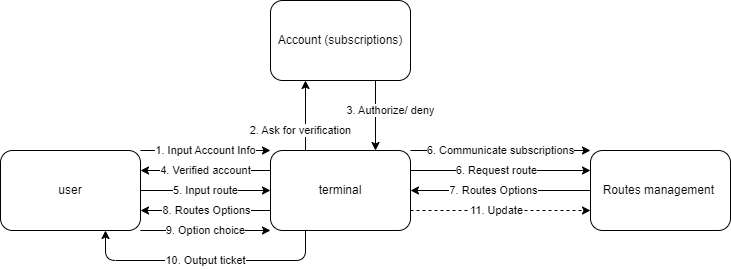
\includegraphics[width=\textwidth]{drawings/decision4_drawings/account_functional.png}
    \caption{Account Management Interaction for single-ticket.}
    \label{fig:account_management_ticket}
\end{figure}
\subsection*{Pros}

\begin{itemize}[noitemsep]
    \item \textbf{Modular Architecture:} The separation of subscription management and route optimization into distinct modules enhances the system's modularity, making it easier to maintain, update, or replace parts of the system without affecting others.
    \item \textbf{Scalability:} Designed with scalability in mind, allowing for easy addition and management of new subscriptions or renewal of existing ones, which can accommodate growing passenger demands and evolving business requirements.
    \item \textbf{Reduced Risk of System-wide Failures:} By distributing functionalities across different systems or modules, the impact of a failure in one component is limited, reducing the risk of system-wide outages and improving overall system reliability.
    \item \textbf{Flexibility in Passenger Authentication:} Supports various means of passenger authentication (e.g., magnetic card, smartphone app), offering flexibility and convenience for passengers to access their subscriptions and travel seamlessly.
\end{itemize}

\subsection*{Cons}

\begin{itemize}[noitemsep]
    \item \textbf{Increased System Interactions:} The decoupled nature of the system requires more interactions between separate modules (e.g., subscription verification and route optimization), which can increase the complexity of integration and potentially lead to higher latency in response times.
    \item \textbf{Integration Complexity:} Ensuring seamless communication and data consistency between different modules can introduce additional complexity in system integration and require more sophisticated coordination mechanisms.
    \item \textbf{Higher Overhead:} Managing separate systems for subscription and route optimization may lead to higher operational overhead in terms of both system resources and administrative efforts to maintain multiple components.
\end{itemize}

\subsection*{Option 2: Integrated Subscription-Route Optimization Service}
The Integrated Subscription-Route Optimization Service (IS-ROS) combines the functionality of subscription management and route optimization into a single service. 
\subsubsection*{Pros}
\begin{itemize}[noitemsep]
    \item \textbf{Performance} Streamlines the process by combining two functionalities, potentially reducing response time for route optimization.
    \item \textbf{Reduced Interactions between systems} Simplifies the architecture by reducing the number of interactions between separate systems.
\end{itemize}
\subsubsection*{Cons}
\begin{itemize}[noitemsep]
    \item \textbf{Increased Complexity within Single Module} Increases complexity within a single system, which may require more resources to develop and maintain.
    \item \textbf{Failures have larger impact} May lead to higher dependency on a single system, which can be a point of failure if the system goes down.
\end{itemize}

\subsection*{Option 3: Include a Single-Ticket management module}
Abstractly, a single ticket can be seen as an account that expires once the journey is completed. As an account, it is linked to a passenger via their personal data, if it is related to a booking or via 
an anonymous user ID if it is not.
Its temporary nature though causes different needs for information storage and flow, as updates for single tickets occurs often.
Hence the need for a separated module and a related database.

\subsection*{Decision}
We decided to pick Option 1. The increased concern for scalability, caused by event 1, points clearly to the listed pros of this option. Furthermore, the focus on modularity
gives us easy maintenability, which is important for the TRIP owner.
Performance in this case doesn't seem to be that central, as optimization of routes should be precomputed and cached, given that timetables should not change often and that subscription have relatively long lasting periods.
With our option, we still have the flexibility to assign more computational or data access resources to the module who needs them the most.
We also include Option 3, as we think Single Tickets remain central to achieve the Usability required by stakeholders who are less familiar with technology such as smartphone apps or are travelling only occasionally.

\subsection*{Consequences}
\subsection*{Positive Consequences}

\begin{itemize}[noitemsep]
    \item \textbf{Enhanced Scalability:} Modular design facilitates easy scaling and integration of new features.
    \item \textbf{Improved Maintainability:} Simplifies updates and troubleshooting, allowing for technology-specific optimizations within each module.
    \item \textbf{Reduced System-wide Failure Risk:} Isolates failures to individual modules, enhancing overall system reliability.
    \item \textbf{Enhanced Usability for Single-Ticket buyers:} A specific module allows good handling of their needs with a high performance DB.
\end{itemize}

\subsection*{Negative Consequences}

\begin{itemize}[noitemsep]
    \item \textbf{Increased System Complexity:} Necessitates sophisticated coordination and integration, potentially introducing latency.
    \item \textbf{Higher Initial Costs:} Development and maintenance of separate modules may lead to higher initial and operational costs.
    \item \textbf{Data Consistency Challenges:} Requires robust synchronization mechanisms to ensure data consistency across modules.
\end{itemize}

The account management module is included in the functional view of the system, communicating with the tycoons to updated them on new subscriptions, with the database to keep the account data up to date and with the terminal to allow 
the purchase of new subscriptions and the verification via magnetic card or other means.